\documentclass{ecnreport}
\setlength{\parindent}{0cm}

\stud{Option Robotique, Control \& Robotics master}
\topic{Advanced Robot Programming}

\def\maze{\texttt{ecn::Maze}~}

\begin{document}

\inserttitle{Advanced Robot Programming  Labs \newline C++ Programming}

\insertsubtitle{Maze generation and solving}

\newcommand{\involves}[1]{
\item {\bf C++ skills:} #1
}

\newcommand{\aitip}[1]{
\item {\bf AI tips:} #1
}

\section{Content of this lab}

In this lab you will use and modify existing code in order to generate and solve mazes. As shown in \Fig{maze2}, the goal is to generate 
a maze of given dimensions (left picture) and to use a path planning algorithm to find the shortest path from the upper left to the lower right corners (right picture).

\begin{figure}[h]\centering
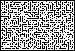
\includegraphics[width=.4\linewidth]{maze} \quad \quad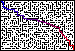
\includegraphics[width=.4\linewidth]{maze_cell}
\caption{$51\times 75$ maze before (left) and after (right) path planning.}
\label{maze2}
\end{figure}

The lab was inspired by \link{https://www.youtube.com/watch?v=rop0W4QDOUI}{this Computerphile video}.\\

We use the classical mix of Git repository and CMake to download and compile the project:
\begin{center}
 \texttt{mkdir build} $\rightarrow$ \texttt{cd build} $\rightarrow$ \texttt{cmake ..} $\rightarrow$ \texttt{make}
\end{center}
The program can the be launched.


\section{Required work}

Four programs have to be created: 
\begin{enumerate}
 \item Maze generation
 \item Maze solving through A* with motions limited to 1 cell (already quite written)
 \item Maze solving through A* with motions using straight lines
 \item Maze solving through A* with motions using corridors
\end{enumerate}

As in many practical applications, you will start from some given tools (classes and algorithm) and use them inside your own code.\\
As told during the lectures, understanding and re-using existing code is as important as being able to write something from scratch.

\section{Maze generation}

The \link{https://en.wikipedia.org/wiki/Maze_generation_algorithm}{Wikipedia page} on maze generation is quite complete
and also proposes C-code that generates a perfect maze of a given (odd) dimension. A perfect maze is a maze where there is one and only 
one path between any two cells.

Create a \texttt{generator.cpp} file by copy/pasting the Wikipedia code and modify it so that:
\begin{itemize}
 \item It compiles as C++.
 \item The final maze is not displayed on the console but instead it is saved to an image file 
 \item The executable takes a third argument, that is the percentage of walls that are randomly erased in order to build a non-perfect maze.
\end{itemize}
A good size is typically a few hundred pixels height / width. To debug the code, 51 x 101 gives a very readable maze.

The \maze class (\Sec{mazeClass}) should be used to save the generated maze through its \texttt{Maze::dig} method that removes a wall at a given (x,y) position.
It can also save a maze into an image file.


\section{Maze solving}

The given algorithm is described on \link{https://en.wikipedia.org/wiki/A*\_search\_algorithm\#Pseudocode}{Wikipedia}. It is basically a graph-search algorithm that
finds the shortest path and uses a heuristic function in order to get some clues about the direction to be favored.

In terms of implementation, the algorithm can deal with any \texttt{Node} class that has the following methods:
\begin{itemize}
 \item \texttt{vector<unique\_ptr<Node>> Node::children()}: returns a \texttt{vector} of smart pointers\footnote{The use of smart pointers (here \texttt{unique\_ptr}) is detailed in \Sec{smart}} to the children (or neighboors) of the considered
 element
 \item \texttt{int distToParent()}: returns the distance to the node that generated this one
 \item \texttt{bool is(const Node \&other)}: returns true if the passed argument is actually the same point
 \item \texttt{double h(const Node \&goal)}: returns the heuristic distance to the passed argument
 \item \texttt{void show(bool closed, const Node \& parent)}: used for online display of the behavior
 \item \texttt{void print(const Node \& parent)}: used for final display
\end{itemize}


While these functions highly depend on the application, in our case we consider a 2D maze so some of these functions are already implemented in, as seen in \Sec{ptClass}:
\begin{itemize}
 \item For the first exercice, only the \texttt{children} method is to write.
 \item The second one adds the \texttt{distToParent} method.
 \item The last one adds the \texttt{show} and \texttt{print} methods.
\end{itemize}



\subsection{A* with cell-based motions}

The first A* will use cell-based motions, where the algorithm can only jump 1 cell from the current one.

The file to modify is \texttt{solve\_cell.cpp}.
At the top of the file is the definition of a \texttt{Position} class
that inherits from \texttt{ecn::Point} in order not to reinvent the wheel (a point has two coordinates, it can compute the distance to
another point, etc.).

The only method to modify is \texttt{Position::children} that should generates the neighboors of the current point.
The parent node is likely to be in those neighboors, but it will be removed by the algorithm. 

\subsection{A* with line-based motions}

Copy/paste the \texttt{solve\_cell.cpp} file to \texttt{solve\_line.cpp}.\\

Here the children should be generated so that a straight corridor is directly followed (ie children can only be corners, intersections or dead-ends).
A utility function \texttt{bool is\_corridor(int, int)} may be of good use.\\

The distance to the parent may not be always 1 anymore. As we know the distance when we look for the neighboor nodes, a good thing would be to store it 
at the generation by using a new Constructor with signature \texttt{Position(int \_x, int \_y, int distance)}.\\

The existing \texttt{ecn::Point} class is already able to display lines between two non-adjacent points (as long as they are on the same horizontal or
vertical line). The display should thus work directly.

\subsection{A* with corridor-based motions}

Copy/paste the \texttt{solve\_line.cpp} file to \texttt{solve\_corridor.cpp}.\\

Here the children should be generated so that any corridor is directly followed (ie children can only be intersections or dead-ends, but
not simple corners).
A utility function \texttt{bool is\_corridor(int, int)} may be of good use.\\

The distance to the parent may not be always 1 anymore. As we know the distance when we look for the neighboor nodes, a good thing would be to store it 
at the generation by using a new Constructor with signature \texttt{Position(int \_x, int \_y, int distance)}. \\

The existing \texttt{Point::show} and \texttt{Point::print} methods are not suited anymore for this problem. Indeed, the path from a point to its parent 
may not be a straight line. Actually it will be necessary to re-search for the parent using the same approach as to generate the children.\\

For this problem, remember that by construction the nodes can only be intersections or dead-ends. Still, the starting and goal positions may 
be in the middle of a corridor. It is thus necessary to check if a candidate position is the goal even if it is not the end of a corridor.

\section{Comparison}

Compare the approaches using various maze sizes and wall percentage.
If it is not the case, compile in \texttt{Release} instead of \texttt{Debug} and enjoy the speed improvement.\\

The expected behavior is that mazes with lots of walls (almost perfect mazes) should be solved must faster with the corridor, then line, then cell-based approaches.\\
With less and less walls, the line- and cell-based approaches should become faster as there are less and less corridors to follow.

\appendix

\section{Provided tools}

\subsection{The \maze class}\label{mazeClass}

This class interfaces with an image and allows easy reading / writing to the maze. 

\paragraph{Methods for maze creation}
\begin{itemize}
 \item \texttt{Maze(std::string filename)}: loads the maze from the image file
 \item \texttt{Maze(int height, int width)}: build a new maze of given dimensions, with only walls
 \item \texttt{dig(int x, int y)}: write a free cell at the given position
 \item \texttt{save()}: saves the maze to \texttt{maze.png} and displays it
\end{itemize}

\paragraph{Methods for maze access}
\begin{itemize}
 \item \texttt{int height()}, \texttt{int width()}: maze dimensions
 \item \texttt{int isFree(int x, int y)}: returns true for a free cell, or false for a wall or invalid (out-of-grid) coordinates
\end{itemize}

\paragraph{Methods for maze display}
\begin{itemize}
 \item \texttt{write(int x, int y, int r, int g, int b, bool show = true)}\\
    will display the (x,y) with the (r,g,b) color and actually shows if asked
 \item \texttt{passThrough(int x, int y)}: write the final path, color will go automatically from blue to red. 
 Ordering is thus important when calling this function
 \item \texttt{saveSolution(std::string suffix)}: saves the final image
\end{itemize}

\subsection{The \texttt{ecn::Point} class}\label{ptClass}

This class implements basic properties of a 2D point:

\begin{itemize}
 \item \texttt{bool is(Point)}: returns true if both points have the same x and y coordinates
 \item \texttt{double h(const Point \&goal)}: heuristic distance, may use Manhattan
 ($|x-\texttt{goal}.x| + |y-\texttt{goal}.y|$) or classical Euclidean distance.
 \item \texttt{void show(bool closed, const Point \& parent)}: draws a straight line between the point and its parent, that
 is blue if the point is in the closed set or red if it is in the open set.
 \item \texttt{void print(const Point\& parent)}: writes the final path into the maze for display, also considers a straight line
\end{itemize}
All built classes should inherit from this class. The considered maze is available through the static member variable \texttt{ecn::maze} and can thus
be accessed from the built member functions.

\section{Pointers and smart pointers}\label{smart}

During an A* algorithm, a lot of nodes are created, deleted and moved between the open and the closed set.
This makes it necessary to create the nodes on the heap and manipulate only pointers. 
In our case, new nodes are created in when calling the \texttt{children()} method, while they are deleted by the algorithm
itself if needed. In order to avoid memory leaks, we will use smart pointers.\\

Assuming that a new position can be created from its coordinates, a new position may be created with:
\begin{itemize}
\item \texttt{Position p(x, y);} for an actual position
 \item \texttt{Position* p = new Position(x, y);} for a raw pointer
 \item \texttt{std::unique\_ptr<Position> p(new Position(x, y);} for a unique ptr
\end{itemize}

As the \texttt{children()} method is supposed to return a \texttt{std::vector} of pointers, the corresponding syntax may be as follows:
\begin{center}\cppstyle
\begin{lstlisting}
typedef std::unique_ptr<Position> PositionPtr;
std::vector<PositionPtr> children()
{
    std::vector<PositionPtr> generated;
    while(..)   // whatever method we use to look for children
    {
    
        // assuming that we found a child at (x,y)
        generated.push_back(std::make_unique<Position>(x,y)));
    }
    return generated;
}
\end{lstlisting}
\end{center}
Here the generated children are directly put inside the vector, which is returned at the end. The smart pointer keeps track 
of the allocated memory and the A* algorithm can decide to keep it or not, knowing that the memory will be managed accordlingly.


\end{document}
